\section{Cohesive sediment}\label{ch:cohesive}\footnote{This chapter has been written by D. Phan van Bang, Lan and Villaret}


\subsection{Introduction}
\subsubsection{Sediment bed composition}
The non-cohesive sediment composition is represented by a finite number of
classes, each characterized by its mean diameter, grain density and constant
settling velocity. The fine cohesive particles made of silt and clay present
specific properties (flocculation, consolidation) for a grain diameter less
than a limiting value of about 60 $\mu$m.

For cohesive sediments, the bed is generally non-uniform: as a result of
underweight consolidation, the bed becomes stratified, with density
increasing with distance from the surface. The top layer is therefore made
of soft mud which can be viewed as the active layer. It is indeed eroded
under the action of regular currents, while the sediment in suspension will
be deposited in this first layer. The bottom consolidated layers present
higher resistance and can only be eroded under extreme events. This vertical
stratification of the bed is therefore a key issue, which controls the
amount of material to be put in suspension. 

Cohesive sediments are transported only in suspension (no bedload), such
that the Exner equation for the bed evolution is no-longer solved. The bed
evolution is obtained as a mass balance between the erosion and deposition
fluxes, which are calculated in \sisyphe using the Krone and Partheniades
laws: the erosion flux need specific treatment in order to correctly account
for the vertical increase in the bed shear strength as the bed gets eroded.

The effect of flocculation can be represented in the model by specifying a
higher settling velocity parameter which can be an order of magnitude
greater than the individual or primary particle settling velocity. More
physically based relation have been programmed in the 3D library of \telddd
following the method of Van Leussen (1994).

The model presents different options to represent the effect of
consolidation: different schemes can be used. In a so-called iso-pycnal
scheme, the bed is represented by a number of layers of increasing
concentration. The concentration of each layer is fixed, while their
thickness varies in time as the bed undergoes erosion/deposition/consolidation. This scheme is used in a semi-empirical
model, originally developed by Villaret and Walther (2008). A new scheme
developed by Lan Anh Van (2012) is based on the Gibson's theory (Gibson et
al, 1967, 1981). An other third scheme has been implemented which is similar
to the Gibson consolidation model developed in \telddd by LeNormand (1993).
In this third model, the bed is discretised in layers of given thicknesses
and time-varying concentrations. This third model has been shown to be
unstable and CPU time-consuming (cf. Van, 2012). 

This chapter is organized as follows. Section 2 presents the initialization of cohesive sediment
properties. Section 3 concentrates on the erosion/deposition and Section 4 on the
consolidation. Appendix 1 gives a list of keywords for cohesive applications and user-subroutine. In
Appendix 2, the Gibson equation is derived for consolidation modelling.

\subsection{Initialization of cohesive sediment}

\subsubsection{Sediment properties}
\subsubsection*{Non cohesive/cohesive sediment}
Fine sediment particles of diameters less than 60 $\mu$m present complex
cohesive properties which affect the sediment transport processes.
For non-cohesive sediments (D$_{50}>60\mu$m), the grain diameter
and grain density $\rho_s$ are the key parameters which determine its
resistance to erosion, settling velocity and sediment transport rate. Non
cohesive material are generally made of quartz, such that the density of
sand particles is constant and equal to 2650 kg/m$^{3}$. 

For cohesive sediments (D$_{50}< 60 \mu$m), the primary grain
diameter is no longer the key sediment parameter. Due to electro-static
attractive forces (van der Waals), individual particles tend to form floc.
Their size can be an order of magnitude greater than the initial particle
diameter, while the floc density decreases: the floc parameters (size and
density) are more relevant to compute the terminal velocity. 

The settling velocity of cohesive particles therefore depends on the
suspended sediment concentration as well as to other physico-chemical
properties (pH, salinity, cations for instance) of the suspension which
influence the flocculation process. The effect of turbulence level
determines also the flocculation state. The critical bed shear strength
depends on the consolidation state or age of the sediment bed (Migniot,
1968).

\begin{bclogo}[couleur = blue!10, arrondi = 0.10, logo = \bcattention]{\textsf{Attention}}
The separation value at $60\mu$m to discriminate non-cohesive from
cohesive sediment is conventional (UK classification). The value is
different depending on the country ($63\mu$m in Netherlands, $75\mu$m in USA
as pointed by Winterwerp and Van Kesteren, 2004). Moreover, aggregation of
flocs can lead to the formation of macro-flocs larger than $100\mu$m.
\end{bclogo}

We consider in Sections 3-5, the simpler case of uniform, cohesive sediments,
characterized by one single value for the primary grain size $D_{50}$ and
density $\rho_s=2650$ kg/m$^{3}$ for quartz particles, which is
transported in suspension (no bedload). In \sisyphe, the effect of
flocculation is represented by the choice of settling velocity considered to
be constant (for simplicity). More physically based relations will be
implemented in the future. The effect of consolidation is modeled through
physical as well as empirically-based models.

\medskip
\begin{bclogo}[couleur=blue!10,arrondi=0.1, logo=\bcinfo]{Keywords}
In the \sisyphe steering file, the physical properties of the sediment are
defined:
\begin{itemize}
\item {\ttfamily COHESIVE SEDIMENT = YES} ({\ttfamily = NO}, default option)
\item {\ttfamily SEDIMENT DIAMETERS} ($D_{50} > 0.00006$ m, for non-cohesive sediment)
\item {\ttfamily SEDIMENT DENSITY} ($\rho_s = 2650$ Kg/m$^3$, default value)
\item {\ttfamily SETTLING VELOCITIES}
\item {\ttfamily SUSPENDED LOAD = YES} ({\ttfamily = NO}, default option)
\item {\ttfamily BED LOAD = NO} ({\ttfamily = YES}, default option)
\end{itemize}
\end{bclogo}

\begin{bclogo}[couleur = blue!10, arrondi = 0.10, logo = \bcattention]{\textsf{Attention}}
\begin{enumerate}
\item The settling velocity needs to be specified, if not, it will
be calculated by the Stokes law as a function of the individual particle
diameter in subroutine \texttt{vitchu\_sisyphe.f}. As a result of flocculation, the
settling velocity can be approximately an order of magnitude greater. 

\item Both key words \texttt{SUSPENDED LOAD = YES}, \texttt{BED LOAD = NO} are
set automatically, in order to be consistent with the selected type of
sediment, when \texttt{COHESIVE SEDIMENT = YES}
\end{enumerate}
\end{bclogo}

\subsubsection{Sediment bed structure}

The cohesive sediment bed properties are generally not uniform: as a result
of self-weight consolidation, the top layer is made of freshly deposited
mud. This soft layer represents the active layer, which is regularly eroded
under the action of regular currents in mean flow conditions. The
concentration increases with distance from the surface, whereas its
resistance to erosion increases. The vertical bed structure determines both
the erosion flux and the resulting bed evolution. 

In \sisyphe, cohesive sediment bed can be represented by a fixed number
\texttt{NOMBLAY} of layers of iso-pycnal (constant concentrations). The number of
layers is fixed with maximum number up to $20$. Each layer is represented by a
constant concentration. The concentration of each layer is generally fixed
and specified by keyword \texttt{MUD CONCENTRATION PER LAYER} expressed in kg/m$^3$. It
may also vary in space and time (see consolidation model 3).

\begin{figure}[ht]
\label{fig:1}
\begin{center}
\begin{tabular}{c}
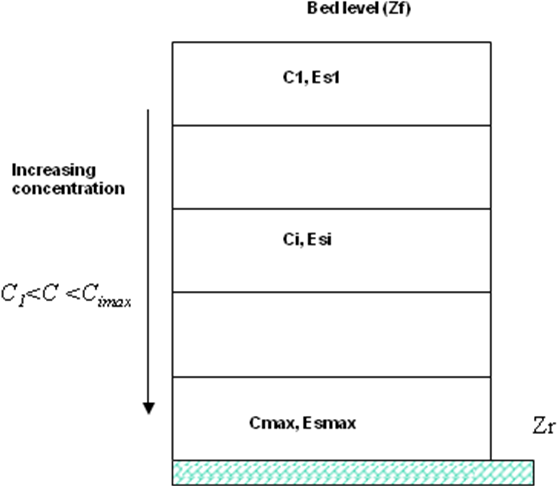
\includegraphics[scale=1.0]{graphics/vertical_bed_structure.png} %&
\end{tabular}
\caption{Schema of vertical bed structure. \texttt{NOMBLAY} is the number of layers.}
\end{center}
\end{figure}

\subsubsection{Initialization of the sediment bed structure}

The initial concentrations (CONC\_VASE (j)) are generally specified by
keywords.\newline
The initial layer thicknesses are specified in user-subroutine
init-compo-coh.f. It is called by subroutine init\_mixte.f which just checks
if the sum of all layers is equal to the total bed thickness as specified by
the initial bathymetry Zf and rigid bed Zr :

\begin{equation*}
Z_{f} (i)-Z_{r} (i)=\sum\limits_{j=1,NOMBLAY}Es(i,j) 
\end{equation*}%
(unknown char)\hspace{5mm} i is the number of point,\newline
(unknown char)\hspace{5mm} j the number of layer.\newline
(unknown char)\hspace{5mm} Zf: the bed level\newline
(unknown char)\hspace{5mm} Zr: the non-erodible bed level

Each layer j ( $1\leq j\leq NOMBLAY$) is defined by its concentration C$_{s}$%
, thickness E$_{s}$ and mass per surface area M$_{s}$, which depends on both
layer concentration and thickness, such that

M$_{s}$(i, j)= C$_{s}$ (j) E$_{s}$(i,,j),\newline
(unknown char)\hspace{5mm} Ms is the mass per unit surface area (Kg/m$^{2}$),%
\newline
(unknown char)\hspace{5mm} Cs is the concentration (kg/m3),\newline
(unknown char)\hspace{5mm} Es, the layer thickness.

For particular application, the bed concentrations C$_{S}$ (i, j) can be
also allowed to vary from point to point. The initial distribution can be
specified in subroutine init\_compo-coh.f. \newline
Key words\newline
$\neg$\hspace{5mm} `NUMBER OF LAYERS OF THE CONSOLIDATION MODEL' \newline
o\hspace{5mm} NCOUCH\_TASS = 1 (default value) should be less than the
maximum number of layers (NLAYMAX = 20)\newline
$\neg$\hspace{5mm} 'MUD CONCENTRATION PER LAYER' in (Kg/m$^{3}$ ): CONC\_VASE

Remarks\newline
$\neg$\hspace{5mm} The keywords `NUMBER OF BED LOAD MODEL LAYERS' and
`NUMBER OF LAYERS OF THE CONSOLIDATION MODEL' are essentially the same
except that the default values are different. For cohesive sediments, it is
possible to have only one uniform layer, whereas for sand grading algorithm
we need at least 2 layers (the active layer and the substratum).

The subroutine lecdon.f specifies at the end NOMBLAY = NCOUCH\_TASS\newline

\subsection{Erosion/deposition properties}

\subsubsection{Transport in suspension}

Transport equation

Fine cohesive sediments are transported in suspension. The two-dimensional
(2D) model solves a two-dimensional (2D) transport equation for the
depth-averaged suspended sediment transport concentration C, which is
derived by depth-integration of the 3D classical transport/diffusion
equation.

\begin{equation*}
X=\overline{x} =\frac{1}{h} \int\nolimits_{Z_{f} }^{Z_{s} }x(z)dz 
\end{equation*}%
\hspace{5mm} \hspace{5mm} \hspace{5mm} (1)\hspace{5mm}

where h =Z$_{s}$-Z$_{f}$ is the water depth, assuming the bed-load layer
thickness to be small.\newline
After simplification of the advection terms and using the continuity
equation, the following approximate depth-averaged transport equation can be
solved in its non-conservative form:

\begin{equation*}
\frac{\partial C}{\partial t}+\underbrace{U\frac{\partial C}{\partial x}+V%
\frac{\partial C}{\partial y}}Adv=\underbrace{\frac{1}{h}\left[ \frac{%
\partial }{\partial x}\left( h\epsilon _{s}\frac{\partial C}{\partial x}%
\right) +\frac{\partial }{\partial y}\left( h\epsilon _{s}\frac{\partial C}{%
\partial y}\right) \right] }Diff+\frac{(E-D)}{h}
\end{equation*}%
\hspace{5mm} \hspace{5mm} (2)\hspace{5mm} \newline
(unknown char)\hspace{5mm} U and V are the depth-averaged convective flow
velocities in the x and y directions,\newline
(unknown char)\hspace{5mm} E and D are respectively the erosion and
deposition fluxes at the bed and represent the exchange terms between the
suspension and the sediment bed. They are defined at the interface between
the bed and the suspension.

Units\newline
In SISYPHE, the volume concentration is the main variable: such that E and D
are expressed in m/s \newline
However, the user can choose mass concentration for graphic printouts, by
use of keyword `MASS CONCENTRATION'.\newline
The relation between volume concentration C and mass concentration C$_{s}$
(Kg/m$^{3}$) is: C$_{s}$ = $\rho$$_{s}$ C, where $\rho$$_{s}$ is the solid
density ($\rho$$_{s}$ = 2650 Kg/m$^{3}$)\newline
Convection\newline
For non cohesive sediments, the convective velocity generally differs from
the depth-averaged velocity (issued from Telemac-2d). A correction term is
applied on the depth-averaged mean velocity to account for the fact that
most sediments is transported near the bed. This correction term is
expressed as a function of the Rouse parameter as explained in the
user-manual (cf. Report H-P74-2012-02004-EN). \newline
For fine cohesive sediments, the Rouse parameter

\begin{equation*}
R=\frac{W_{s} }{\kappa u_{*}} 
\end{equation*}%
(where W$_{s}$ is the settling velocity, $\kappa$ , the von Karman constant (%
$\kappa$=0.4), and u$_{*}$ the friction velocity ) is generally less than
one and the sediment can be regarded as fairly uniformly distributed in the
vertical. The convection velocity can be taken as the depth-averaged flow
velocity.\newline
Diffusion\newline
The horizontal diffusion terms can be set to zero by use of keyword
`DIFFUSION' = NO.\newline
According to the choice of the parameter `OPDTRA' (keyword), the diffusion
terms in (2) can be simplified and equation (2) becomes :

\begin{equation*}
\frac{\partial C}{\partial t} +U_{} \frac{\partial C}{\partial x} +V\frac{%
\partial C}{\partial y} =\left[ \frac{\partial }{\partial x} \left( \epsilon
_{s} \frac{\partial C}{\partial x} \right) +\frac{\partial }{\partial y}
\left( \epsilon _{s} \frac{\partial C}{\partial y} \right) \right] +\frac{%
(E-D)}{h} 
\end{equation*}
(3)

Keywords\newline
(unknown char)\hspace{5mm} `correction on convection velocity' (NO = Default
value). \newline
(unknown char)\hspace{5mm} `MASS CONCENTRATION' = YES (NO, default value)

Treatment of advection terms

The choice of the numerical scheme is based on keyword (`TYPE OF
ADVECTION'). The following finite elements methods available are:\newline
-\hspace{5mm} 1. Method of characteristics \newline
o\hspace{5mm} Main advantages : unconditionally stable and monotonous\newline
o\hspace{5mm} Diffusive for small time steps\newline
o\hspace{5mm} Not mass conservative\newline
-\hspace{5mm} 2. Method Streamline Upwind Petrov Galerkin (SUPG)\newline
o\hspace{5mm} Courant number criteria\newline
o\hspace{5mm} Not mass conservative\newline
o\hspace{5mm} Less diffusive for small time steps\newline
-\hspace{5mm} 3 or 4. Conservative N-scheme (similar to finite volumes)%
\newline
o\hspace{5mm} solves the continuity equation under its conservative form%
\newline
o\hspace{5mm} (recommended when the correction on convection velocity is
accounted for)\newline
o\hspace{5mm} Courant number limitation (sub iterations are included to
reduce the time step\newline
-\hspace{5mm} 13, 14 are the same as 3 and 4 but here adapted to the
presence of tidal flats based on positive water depth algorithm \newline
-\hspace{5mm} 5. Distributive schemes (PSI): like N scheme 4, but non-linear
ie the fluxes are corrected according to the tracer value itself. This
relaxes the courant number criteria and it is also less diffusive than
scheme 4 and 14. The CPU time is however increased. This method does not
apply for tidal flats.

It is therefore recommended to use scheme 4 or 14 (if tidal flats) as a good
compromise (accuracy/computational time)\newline
Keywords\newline
The following keywords determine the numerical scheme options, choice of
advection scheme, accuracy of solver, coefficient of implicitation \dots . 
\newline
(unknown char)\hspace{5mm} `TETA SUSPENSION'(TETA\_SUSP = 1, by default) 
\newline
(unknown char)\hspace{5mm} `TYPE OF ADVECTION'(=1, default option:
characteristics)\newline
o\hspace{5mm} The method of characteristics is non-conservative\newline
o\hspace{5mm} Use method 4 (or 14 in the presence of tidal flats) to check
mass continuity

(unknown char)\hspace{5mm} `SOLVER FOR SUSPENSION'(=3, conjugate gradient,
by default)\newline
(unknown char)\hspace{5mm} `PRECONDITIONING FOR SUSPENSION'\newline
(unknown char)\hspace{5mm} `SOLVER ACCURACY FOR SUSPENSION' (= 10$^{-8}$, by
default)

It is important to have a small value here, when working with volume
concentration \texttt{<}\texttt{<}\texttt{<}1\newline
(unknown char)\hspace{5mm} `MAXIMUM NUMBER OF ITERATIONS FOR SOLVER FOR
SUSPENSION'(=50, per default)

It is important to have a small value here, when working with volume
concentration \texttt{<}\texttt{<}\texttt{<}1\newline
(unknown char)\hspace{5mm} OPTION FOR THE DISPERSION( =1, constant
dispersion coefficient per default)\newline
(unknown char)\hspace{5mm} DISPERSION ALONG THE FLOW =10$^{-2}(unknown char)%
\hspace{5mm} DISPERSION ACROSS THE FLOW =10^{-2}$

See also : \newline
(unknown char)\hspace{5mm} `MATRIX-VECTOR PRODUCT', `MATRIX STORAGE\dots '

The user should refer to the ``Sisyphe.dico'' file, if he would like to
modify some of the numerical options and parameters. See also Hervouet
(2007, chapter 6).

\subsubsection{Erosion flux for cohesive sediment}

Uniform bed\newline
The classical Partheniades formula is applied for cohesive sediments.
Assuming the bed to be uniform: \hspace{5mm}

\begin{equation*}
\left. 
\begin{array}{l}
E=M\left[ \left( \frac{u_{^*} }{u_{*_e}} \right)^2 -1\right]
\;\;for\quad\,u_{*} >u_{*_e} \;\;\, \\ 
E=0\;\;for\;\;u_{*} <u_{*_e}%
\end{array}
\right\} \;\;(4) 
\end{equation*}%
\hspace{5mm} where u$_{*}$ is the friction velocity related to skin
friction, u$_{*e}$ is the critical shear stress velocities for erosion. 
\newline
(unknown char)\hspace{5mm} u$_{*ce}$ is the critical erosion velocity, 
\newline
(unknown char)\hspace{5mm} u* the friction velocity, defined as a

\begin{equation*}
u_{*} =\sqrt{\frac{\tau ^{\prime }_{} }{\rho } } 
\end{equation*}%
(unknown char)\hspace{5mm} $\tau$' the shear stress corrected for skin
friction,\newline
(unknown char)\hspace{5mm} $\rho$ the fluid density.

The empirical coefficient M is a dimensional coefficient. The Partheniades
coefficient M is specified in the steering file (in Kg/m$^{2}$/s). The
erosion rate is expressed in m/s, by converting the M coefficient to m/s
(subroutine lecdon.f).

Non uniform bed\newline

\begin{equation*}
\tau _{ce} =\rho u_{_{*ce} }^{2} \approx C^{\beta } 
\end{equation*}%
In the multi-layer model, the critical erosion shear stress increases as the
mud concentration increases. The following semi-empirical formulae have been
established (e.g. Migniot, 1968):\newline
(unknown char)\hspace{5mm} $\tau$$_{ce}$ is the critical erosion bed shear
stress, \newline
(unknown char)\hspace{5mm} C the mud concentration, \newline
(unknown char)\hspace{5mm} $\beta$ an empirical coefficient.

In the multi-layer model, each layer is characterized by its density and
critical bed shear stress. \newline
The erosion rate of each layer E(j) decreases with distance from the surface.

For each layer j and at each time step, the erosion rate E(j) is calculated
as a function of the difference between the applied bed shear stress and the
critical bed shear strength, using (4). For each E(j)\texttt{>}0, the layer
is erodible.\newline
The mean erosion flux E is determined as the mean erosion rate, averaged
over the eroded depth :

\begin{equation*}
E=\frac{1}{\Delta zer} \int\limits_{0}^{\Delta zer}E(z)dz=\frac{1}{\rho sDt}
\int\limits_{0}^{Dt} dMs 
\end{equation*}%
(unknown char)\hspace{5mm}  dM$_{s}$ is the eroded mass per unit surface
area (Kg/m$^{2}$),\newline
(unknown char)\hspace{5mm} $\Delta$zer is the maximum depth to be eroded, 
\newline
(unknown char)\hspace{5mm} E(z) is the erosion flux (m/s) at distance z from
the bed interface,\newline
(unknown char)\hspace{5mm} Dt, the time step.

Iterative procedure \newline
The potential depth to be eroded is estimated using the iterative procedure
described below and programmed in subroutine suspension\_erosion\_coh.f.%
\newline
At each time step, the top layer is first eroded if E(1)\texttt{>}0. Once it
is empty, the next layer is eroded etc... For each erodible layer j with
erosion rate (E(j) \texttt{>}0), the time interval Dt(j) to erode it
completely is estimated by a simple mass balance from the mass of the layer
Ms(j) :

\begin{equation*}
Dt(j)=\frac{M_{s} (j)}{\rho _{s} E(j)} =\frac{E_{s} (j)*C_{s} (j)}{\rho _{s}
E(j)} 
\end{equation*}
For the first layer (j=1), there are two possibilities: \newline
(unknown char)\hspace{5mm} Dt(1)\texttt{>}Dt : layer 1 is emptied partially :

\begin{equation*}
-C_{s} (1)dE_{s} (1)=\rho _{s} DtE\left( j\right) 
\end{equation*}%
(unknown char)\hspace{5mm} Dt(1)\texttt{<}Dt : layer 1 is emptied completly,
and the next (second) layer can be eroded:

dEs(1)=-Es(1)

The last (non-empty) layer (noted j$_{max}$) to be eroded is obtained by
emptying all successive top layers until :

\begin{equation*}
\sum\limits_{j=1}^{j\max -1} Dt(j)<Dt<\sum\limits_{j=1}^{j\max } Dt(j) 
\end{equation*}
For j$_{max}$, the time left to erode the last layer is

\begin{equation*}
Dt_{\max } =Dt-\sum\limits_{j=1}^{j\max -1} Dt(j) 
\end{equation*}%
The mass potentially eroded during this process is

\begin{equation*}
\overline{M_{s} } =\sum\limits_{j=1}^{j\max -1}M_{s} (j) +\rho _{s}
E(j_{\max } )Dt_{\max } 
\end{equation*}%
The erosion flux (m/s) is therefore estimated{\nobreakspace}: \hspace{5mm}

\begin{equation*}
E=\frac{\overline{M_{s} } }{\rho _{s} Dt} 
\end{equation*}
Keywords\newline
(unknown char)\hspace{5mm} `COHESIVE SEDIMENTS' = YES ( NO; default option),%
\newline
(unknown char)\hspace{5mm} `PARTHENIADES CONSTANT' (M = 10$^{-3}$ Kg/m$^{2}$%
/s, by default),\newline
(unknown char)\hspace{5mm} `CRITICAL EROSION SHEAR STRESS OF THE MUD'
(TOCE\_VASE : $\tau$$_{ce}$ = 0.01 N/m$^{2}$ by default), in N/m$^{2}$

\subsubsection{Deposition flux for cohesive sediment}

The deposition flux is calculated as a function of the near bed
concentration, which in the case of cohesive sediments is considered equal
to the depth-averaged concentration. In the transport equation (3), the
deposition flux is therefore an implicit term, whereas the erosion flux is
explicit.

\begin{equation*}
\left. 
\begin{array}{l}
D=0\qquad\qquad\quad\;\;for\quad\,u_* >u_{*_d} \;\;\, \\ 
D=W_s C\left[ 1-\left( \frac{u_*} {u_{*_d}} \right) ^{2} %
\right] \quad\;for\;\;u_* < u_{*_d}%
\end{array}
\right\} \;\;(5) 
\end{equation*}%
(unknown char)\hspace{5mm} C is the depth-averaged concentration \newline
(unknown char)\hspace{5mm} W$_{s}$ is the settling velocity\newline
(unknown char)\hspace{5mm} U$_{*d}$, the critical deposition velocity which
represents the limiting shear velocity, above which the sediment flocs are
broken and resuspended.

In the case of cohesive sediments, the settling velocity is generally an
order of magnitude greater the settling velocity based on the individual
particle size, as a result of flocculation.\newline
The flocculation process is not yet programmed in Sisyphe and the settling
velocity should be specified by the user as a calibration parameter. \newline
Remark \newline
In Eq(5), the sediment concentration is assumed to be uniform over depth,
which is a reasonable assumption for fine cohesive sediments (W$_{s}$\texttt{%
<}\texttt{<}u*).

Keywords\newline
(unknown char)\hspace{5mm} `CRITICAL SHEAR VELOCITY FOR MUD DEPOSITION'
(VITCD: = 1000 m/s , by default: for no deposition),\newline
(unknown char)\hspace{5mm} `SETTLING VELOCITIES' (By default, W$_{s}$ is
calculated by the model based on the Stokes law and individual particle
diameter)\newline

\subsubsection{Bed evolution}

In the case of cohesive sediments, there is no bed-load. The bed evolution
is only due to the suspension. This is the mass conservation equation to be
solved at each time step:

\begin{equation*}
C_{s} \frac{\partial Z_{f} }{\partial t} +\rho _{s} (E-D)=0 
\end{equation*}%
\hspace{5mm} (6) \newline
(unknown char)\hspace{5mm} Z$_{f}$ is the bottom elevation (m), \newline
(unknown char)\hspace{5mm} C$_{s}$ is the mass concentration of the cohesive
bed which increases from the top layer to the bottom in the multi-layer
discretization of the bed (Kg/m$^{3}$). \newline
(unknown char)\hspace{5mm} E-D is the net sediment flux (m/s), \newline
(unknown char)\hspace{5mm} $\rho$$_{s}$ the solid particles density (Kg/m$%
^{3}$).

The subroutine evol\_susp\_coh.f updates the bed level dZ$_{f}$ and layer
thicknesses E$_{S}$, as well as the mass of mud per layer M$_{s}$.\newline
For uniform bed (NOMBLAY = 1)\newline
The bed is characterized by a single density C$_{s}$= C$_{s}$(1). The bed
evolution at each time step is therefore:

\begin{equation*}
dZ_{f} =\frac{\rho _{s}^{} (D-E)Dt}{C_{s} } 
\end{equation*}
(dZ$_{f}$ \texttt{<} 0 for net erosion and dZ$_{f}$ \texttt{<} 0 for net
deposition).

For non-uniform beds\newline
Two different cases occur. In the case of net deposition (D-E\texttt{>}0),
sediment is deposited in the first top layer C$_{s}$(1):

\begin{equation*}
dZ_{f} =dE_{s} (1)=\frac{\rho _{s}^{} (D-E)Dt}{C_{s} (1)} >0 
\end{equation*}
In the case of net erosion (E-D\texttt{>}0), sediment is eroded layer by
layer dEs(j) \texttt{<}0, from the surface to the bottom dense layer, until
the eroded mass balances the eroded flux:

\begin{equation*}
\sum\limits_{j=1}^{j\max } M_{s} (j)=\rho _{s} (E-D)Dt 
\end{equation*}%
(unknown char)\hspace{5mm} j$_{max}$ is the last layer to be eroded,\newline
(unknown char)\hspace{5mm} M$_{s}$(j) is the total mass per surface area of
layer j :\hspace{5mm}

\begin{equation*}
M_{s} (j)=C_{s} (j)E_{s} (j) 
\end{equation*}

The last layer to be eroded j$_{max}$ is determined in order to satisfy:

\begin{equation*}
\sum\limits_{j=1}^{j\max -1}M_{s}^{n} (j) <\rho _{s} (E^{}
-D)Dt<\sum\limits_{j=1}^{j\max }M_{s}^{n} (j) 
\end{equation*}
Top layers are emptied (dEs (j)= - Es(j) for j=1 up to j$_{max}$-1); the
last layer is eroded up to a the depth dE$_{s}$(jmax)\texttt{<}0 in order to
satisfy mass conservation:

\begin{equation*}
\underbrace{\sum\limits_{j=1}^{j\max -1}M_{s}^{n} (j) -dE_{s} (j\max )C_{s}
(j\max )} erosed\,mass=\rho _{s} (E-D)Dt 
\end{equation*}
The variation of bed elevation is therefore:

\begin{equation*}
dZ_{f} =-\left( \sum\limits_{j=1}^{j\max -1}E_{s}^{n} (j) \right) +dE_{s}
(j\max )<0 
\end{equation*}
The thickness and mass of each layer are updated at the end of each time
step (n+1), from their initial values (n) :

\begin{gather*}
for\,j=1,j_{\max } -1\;\;\left\{ 
\begin{array}{l}
E_{s}^{n+1} s(j)=0 \\ 
M_{s}^{n+1} (j)=0%
\end{array}
\right. \;\; \\
for\,j=j_{\max } \left\{ 
\begin{array}{l}
E_{s}^{n+1} (j_{\max } )=E_{s}^{n} (j_{\max } )+dE_{s}^{} (j_{\max } ) \\ 
M_{s}^{n+1} (j_{\max } )=E_{s}^{n+1} (j_{\max } )*C_{s} (j_{\max } )%
\end{array}
\right.
\end{gather*}

Underneath layers (from j$_{max}$+1 to NOMBLAY) are not eroded and keep
their thickness and mass.

Keywords \newline
$\neg$\hspace{5mm} 'MUD CONCENTRATION PER LAYER' in (Kg/m$^{3}$ )\newline
$\neg$\hspace{5mm} SEDIMENT DENSITY ( $\rho$$_{s}$ =2650 Kg/m$^{3}$)\newline
$\neg$\hspace{5mm} Due to the default value of NOMBLAY for sand grading
effects (NOMBLAY =2),For uniform beds both keywords need to be specified

`NUMBER OF BED LOAD MODEL LAYERS' = 1 \newline
`NUMBER OF LAYERS OF THE CONSOLIDATION MODEL' = 1

\subsubsection{Initial concentrations, boundary conditions}

Initial conditions

The initial concentration for the suspended load can be either imposed
within condim\_susp.f or specified in the steering file through the keyword
`Initial suspension concentrations ' initializes the value of the volume
concentration for each class.\newline
Boundary conditions\newline
For the boundary conditions, the concentration of each class can be
specified in the steering file through keyword: `concentration per class at
boundaries'. It may be also convenient to use keyword `equilibrium inflow
concentration =Yes': the concentration at the entrance of the domain and at
t=0 is set to its equilibrium value, according to the choice of the
`reference concentration formula'. Input concentrations can be also directly
specified (user subroutines: conlit.f).\newline
Equilibrium conditions

The concentrations at the entrance of the domain can be calculated by
SISYPHE assuming equilibrium conditions in order to avoid unwanted
bed-evolution at the entrance of the domain, and also at the first time
step, it is possible to impose the concentration to its equilibrium value,
by activating the keyword `EQUILIBRIUM INFLOW CONCENTRATION'. \newline
The equilibrium (depth-averaged) concentration is then calculated assuming
equilibrium concentration at the bed and a Rouse profile correction for the
F factor.\newline
Keywords\newline
(unknown char)\hspace{5mm} 'INITIAL SUSPENSION CONCENTRATIONS' (C$_{S0}$=0,
default value)\newline
(unknown char)\hspace{5mm} `EQUILIBRIUM INFLOW CONCENTRATION (=NO, default
option)\newline
(unknown char)\hspace{5mm} `CONCENTRATION PER CLASS AT BOUNDARIES' (=0,
default value)

User subroutines\newline
The subroutine condim\_susp.f can be used to specify the initial conditions
for the sediment concentration (see {\S } V.4.2). \newline
The subroutine conlit.f can be used to specify the concentration at the
entrance of the domain.\newline

\subsubsection{Mass conservation algorithm}

The subroutine suspension\_bilan\_coh calculates at each time step the mass
of sediments in the computational domain and ensures that the sum of the
different components is compensated by the fluxes at the liquid boundaries:%
\newline
(unknown char)\hspace{5mm} Mass of sediment in suspension: $M_{1} $

\begin{equation*}
M_{1} =\rho _{s} \iiint\limits_{} c(x,y,z)\delta v =\rho _{s}
\iint\limits_{S} C(x,y)h \delta s 
\end{equation*}%
$_{(unknown char)\hspace{5mm} }$ $_{C}$ is the (depth-averaged) volume
concentration of sediment in suspension \newline
(unknown char)\hspace{5mm} h the water depth, \newline
(unknown char)\hspace{5mm} S is the surface of the computational domain.

In finite elements, each 2D variable is decomposed on basis function $\phi$$%
_{i}$:

\begin{equation*}
M_{1} =\rho _{s} \sum\limits_{i=1,Npoin}C_{i} h_{i} \iint \phi _{i} \delta
s=\rho _{s} \sum\limits_{i=1,Npoin}C_{i} h_{i} S_{i} 
\end{equation*}%
(unknown char)\hspace{5mm} S$_{i}$ are the integral of basis function

(unknown char)\hspace{5mm} Mass of sediment in the bed: $M_{2} $

\begin{equation*}
M_{2} =\iiint\limits_{} C_{s} \delta v=\iint \left(
\int\limits_{Zr}^{Zf}C_{s} \delta z \right) \delta s 
\end{equation*}%
(unknown char)\hspace{5mm} C$_{s}$ is the sediment bed mass concentration. 
\newline
(unknown char)\hspace{5mm} Z$_{f}$ : the bed level\newline
(unknown char)\hspace{5mm} Z$_{r}$ : the non erodible bed level

After discretization of the bed layers into layers of variable thickness E$%
_{s}$ and concentration C$_{s}$ w

\begin{equation*}
M_{2} =\iint \left( \sum\limits_{j=1,Nomblay}M_{s} (j) \right) \delta
s=\sum\limits_{i=1,Npoin}\left[ \sum\limits_{j=1,Nomblay}M_{s} (j) \right]
_{i} S_{i} 
\end{equation*}
Where M$_{si}$ is the total mass per surface area at node i.

\newpage

\subsection{CONSOLIDATION MODEL}

\subsubsection{Theoretical background}

Once the sedimentation process is achieved, a sediment bed is formed. For
non-cohesive bed, no evolution with time will be observed if no erosion or
further sedimentation occurs. For cohesive bed, the concentration will
increase with time as the result of self-weight consolidation or compaction.
Two stages, namely the primary and secondary consolidation (Been and Sills,
1981), are classically considered to explain the progressive compaction of
the cohesive sediment bed with time. As the formed bed resulting from the
sedimentation of mud is very soft, it tends to compact under its
self-weight. During this process, the void ratio tends to diminish so that
pore water is expulsed upward as a result of water incompressibility. The
dynamic of this primary stage of consolidation is therefore controlled by
the permeability of the bed. At the end of the primary consolidation, the
excess pore pressure is fully dissipated (Figure 2) but the cohesive bed
records further compaction. This secondary stage of consolidation is no
longer related to pore pressure but rather to the solid skeleton property.
The secondary consolidation is considered as a result of time effect
(viscous or ageing) in the stress-strain relationship of the soil. Two
effects of time are currently considered in modern soil mechanic: the creep
of the soil (viscous behaviour of cohesive geomaterial) and ageing
(thixotropy of mud). Even through the dynamic of the secondary consolidation
is much slower than the primary consolidation, this stage is important for
long term prediction.


\begin{center}
FIGURE 2: Vertical variation of density and effective stress within the
cohesive sediment bed
\end{center}

Remarks:\newline
1. Most consolidation theories describe the primary consolidation since they
are based on the theory by Terzaghi (1923).\newline
2. The theory by Terzaghi (1923) relates the deformation of the bed to the
permeability and the effective (or solid) stress which is defined as the
difference between the total stress and the pore pressure (principle of
effective stress, Terzaghi, 1923). It corresponds to the stress that is
transmitted directly through the contacts between solid particles. It is
also called osmotic pressure by some authors. Been and Sills (1981)
evidenced the progressive increase of effective stress during the
consolidation process.\newline
3. The theory by Terzaghi (1923) was originally formulated for infinitesimal
strains so that permeability and compressibility could be assumed constant.
The theory was extended for large deformations by Gibson et al (1967, 1981)
as pointed out by Been and Sills (1981).

As an illustration of the process in the water column, Figure 3 proposes a
schematic representation of both, the sedimentation and the consolidation.
In the right side of Figure 3, we present the validity range of the Kynch
theory of sedimentation and of the Gibson theory of large strain
consolidation.\newline
Both theories are unified by Toorman (1996, 1999) which pointed out the fact
that Gibson model can also describe the sedimentation of particle depending
on the choice of closure equations.


\begin{center}
FIGURE 3: Diagram of different processes involved in the settling transport
(left: non-cohesive, right : cohesive)
\end{center}

The general model (Eq.7a, 7b, 7c) proposed by Gibson et al. (1967, 1981)
represents the different stages of consolidation. This equation is based on
a two-phase approach by considering continuity and motion equations for both
fluid and solid phase to obtain the general equation that reads in material
co-ordinate $\zeta $which represents the volume of solids:

\begin{equation*}
\dfrac{\partial e}{\partial t} +\left( \dfrac{\rho _{s} -\rho _{f} }{\rho
_{f} } \right) \dfrac{d}{de} \left( \dfrac{k}{1+e} \right) \dfrac{\partial e%
}{\partial \zeta } +\dfrac{\partial }{\partial \zeta } \left( \dfrac{k}{%
g\rho _{f} (1+e)} \dfrac{d\sigma ^{\prime }}{de} \dfrac{\partial e}{\partial
\zeta } \right) =0 
\end{equation*}%
\hspace{5mm} \hspace{5mm} \hspace{5mm} \hspace{5mm} (7a)\newline
(unknown char)\hspace{5mm} e is the void ratio, \newline
(unknown char)\hspace{5mm} k the hydraulic permeability (in m/s), \newline
(unknown char)\hspace{5mm} $\sigma$' the effective (or solid) stress.

The Gibson equation can be also written in Eulerian framework as:

\begin{equation*}
\dfrac{\partial e}{\partial t} +(1+e)^{2} \left( \dfrac{\rho _{s} -\rho _{f} 
}{\rho _{f} } \right) \dfrac{\partial }{\partial z} \left( \dfrac{k}{(1+e)?}
\right) +\dfrac{(1+e)?}{g\rho _{f} } \dfrac{\partial }{\partial z} \left( 
\dfrac{k}{1+e} \dfrac{\partial \sigma ^{\prime }}{\partial z} \right) =0 
\end{equation*}%
\hspace{5mm} \hspace{5mm} \hspace{5mm} (7b)

This equation is equivalent to:

\begin{equation*}
\dfrac{\partial \phi }{\partial t} -\dfrac{\partial }{\partial z} \left[
\left( k(s-1)\phi +\dfrac{k}{\gamma _{f} } \dfrac{\partial \sigma ^{\prime }%
}{\partial z} \right) \phi \right] =0 
\end{equation*}%
\hspace{5mm} \hspace{5mm} (7c)\newline
(unknown char)\hspace{5mm} $\Phi$ stands for the sediment volume
concentration, \newline
(unknown char)\hspace{5mm} k the hydraulic permeability,\newline
(unknown char)\hspace{5mm} s the density ratio between sediment and fluid (=$%
\rho$$_{s}$/$\rho$$_{f}$), \newline
(unknown char)\hspace{5mm} $\gamma$$_{f}$ the unit weight of fluid (=g$\rho$$%
_{f}$, g being the acceleration of gravity), \newline
(unknown char)\hspace{5mm} z the vertical coordinate (positive upward),%
\newline
(unknown char)\hspace{5mm} t the time.

The equation of Gibson has been widely used in various numerical
consolidation models (Been and Sills (1981), Toorman (1996, 1999),
Bartholomeeusen et al. (2002) for instance) as well as compared with the
experimental results. It has been implemented in Telemac-3d by Lenormand
(1993) or coupled with Telemac-2D by Thiebot (2008). Their method of
resolution has been adapted to SISYPHE by Lan Anh Van (2012) and will be
described in {\S }4.3 and 4.4.

The main difficulty in using the Gibson model is related to the choice for
closing the problem. Two closure equations, for the permeability k and for
the effective stress $\sigma$', is indeed required to obtain the time
evolution of vertical concentration profiles. However, the formulation of
these closure equations remains an open problem and a shared protocol to
determine their parameter values are still lacking as reported by Toorman
(1996, 1999), Bartholomeeusen et al. (2002) or Lan Anh Van (2012). In annexe
9.3, we present the derivation of the Gibson equation in Eulerian coordinate
from a two-phase approach and give the way for obtaining the original Gibson
equation in material coordinate.

\subsubsection{Multi-layer empirical algorithm}

Time evolution\newline
The consolidation effect is reproduced by assuming that the vertical flux of
sediment from layer j to underneath layer j+1 is proportional to the mass of
sediments, Ms (kg/m2), contained in the layer j.

\begin{equation*}
\frac{dM_{s} (j)}{dt} =a_{i} M_{s} (j) 
\end{equation*}
\hspace{5mm} \hspace{5mm} (8)

The transfer mass coefficients a$_{j}$ (in s$^{-1}$) are specified in the
steering file ('MASS TRANSFER PER LAYER'). They correspond to a
characteristic timescale to transfer mass from one layer to another.\newline
This multilayer consolidation model is not related to Gibson equation so
that it should be considered as empirical. Despite its apparent simplicity,
it can qualitatively reproduce an increase of mud bed deposit with time,
while ensuring mass conservation (transfer coefficient of the last bottom
layer is zero). The model results are highly sensitive to the specified
values of the mass transfer coefficients a$_{i}$ which are however difficult
to calibrate. The main advantage of this iso-pycnal formulation relies in
the fact that no vertical grid is required to compute the concentration
evolution of the different layers.

Discretization

The vertical resolution of semi-empirical equation (8) is based on the
multi-layer iso-pycnal model with fixed concentrations. The consolidation is
then reproduced by mass transfer between layers of the model. The transfer
coefficients are fixed for each layer.

The set of mass-transfer coefficients a(j) in (s$^{-1}$) are selected by
calibration, in order to find best agreement of time-varying concentration
profiles between model and experiment. Physically, they represent the
inverse of the residence time per layer. The values a(j) are found to
decrease from top to bottom, as the time scale of consolidation (or
residence time) increases. The mass transfer of the last layer is set to
zero, in order to insure no mass loss at the rigid bed level (impermeability
condition).

Keywords

$\neg$\hspace{5mm} `COHESIVE SEDIMENTS' = YES (default , NO; NO; \dots )%
\newline
$\neg$\hspace{5mm} 'MUD CONSOLIDATION' =YES (=NO, default) \newline
$\neg$\hspace{5mm} ` CONSOLIDATION MODEL' = 1

$\neg$\hspace{5mm} 'NUMBER OF LAYERS OF THE CONSOLIDATION MODEL'
(NOMBLAY=10, default, maximum value is 20 )'\newline
$\neg$\hspace{5mm} 'MUD CONCENTRATION PER LAYER' in Kg/m$^{3}$ (E= 50.;
100.;..,by default )\newline
$\neg$\hspace{5mm} 'MASS TRANSFER PER LAYER' ( = 5.10-5, \dots ..0., by
default)

\subsection{Multi-layer iso-pycnal Gibson's model}

\subsubsection{Theoretical background}

The previous equation presents the advantage of not using a vertical mesh.
However it is not physically based model since it neglects the Gibson
theory. Improvement of this category of model was proposed by Sanchez (1992)
and Thiebot (2008). In these formulations, the sediment flux from one layer
to the other is given not in term of empirical mass transfer coefficient (a$%
_{i}$) but in term of theoretical flux which is given by the Gibson theory.

\subsubsection{Numerical discretization}

\hspace{5mm} The model originally developed by Sanchez (1992) and Thiebot
(2008) is a 1DV sedimentation-consolidation {\guillemotleft }{\nobreakspace}%
multi-layer{\nobreakspace}{\guillemotright } model, based on an original
technique to solve Gibson equation. The advantage of this representation
(9a) if compared with previous one (8) relies on the right hand side term
which relates the mass of sediments, Ms$_{i}$ (kg), to the net flux entering
or leaving the layer. This equation enables therefore to consider the flux
of sedimentation and consolidation as provided by the Gibson theory.

\begin{equation*}
\dfrac{dMs_{i} }{dt} =(F_{i} (t)-F_{i+1} (t))\Delta t\pi r^{2} 
\end{equation*}%
\hspace{5mm} \hspace{5mm} \hspace{5mm} \hspace{5mm} (9a)

In equation (9a), a circular shape (of radius r) is assumed for the surface.
Equivalent to (9a), equation (9b) is expressed in term of layer thickness Es$%
_{i}$ (m), recalling Ms$_{i}$= Cs$_{i}$ $\pi$r$^{2}$ Es$_{i}$$_{.}$. This
last expression becomes independent on the settling column geometry.

\begin{equation*}
\dfrac{dEs_{i} }{dt} =\dfrac{F_{i} (t)-F_{i+1} (t)}{Cs_{i} } 
\end{equation*}%
\hspace{5mm} \hspace{5mm} \hspace{5mm} \hspace{5mm} \hspace{5mm} (9b)

The concentration of the different bed layers Cs(i) are fixed. As the
sedimentation and consolidation progress, the sediment is transferred to the
more concentrated layers, and the thickness of these layers increase as well.

The mass conservation is ensured by requiring at each moment, in each layer, the
equality between the mass contained in a layer at time t + $\Delta t$and the
mass present in this layer at time t in which the outgoing mass was removed
and the incoming mass was added (means the mass that crossed the upper and
lower sections respectively during the time $\Delta t$). The outgoing and
incoming masses are taken into account by sediment flux noted F$_{i}$(t).

\begin{equation*}
F_{i} (t)=\dfrac{(V_{s,i} (t)-V_{s,i-1} (t))C_{i-1} C_{i} }{C_{i-1} -C_{i} } 
\end{equation*}%
\hspace{5mm} \hspace{5mm} \hspace{5mm} \hspace{5mm} \hspace{5mm} (10)

In which V$_{s,i}$ is the falling velocity of the layer i, and can be
defined as:

\begin{gather*}
SiC_{i} \leq C_{gel} V_{s,i} =V_{s,i} (C_{i} )=k(C_{i} )C_{i} \left( \dfrac{1%
}{\rho _{s} } -\dfrac{1}{\rho _{f} } \right) \\
SiC_{i} >C_{gel} V_{s,i} =k(C_{i} )C_{i} \left( \dfrac{1}{\rho _{s} } -%
\dfrac{1}{\rho _{f} } \right) +k(C_{i} )\dfrac{\sigma ^{\prime }(C_{i-1}
)-\sigma ^{\prime }(C_{i} )}{\dfrac{1}{2} (Ep_{i-1} (t)+Ep_{i} (t))}
\end{gather*}
\hspace{5mm} (11)

Where k is the permeability, $\sigma ^{\prime }$is the effective stress, C$%
_{gel}$ the transition concentration between sedimentation and consolidation
schemes (Camenen \& Pham Van Bang, 2011). The closure equation are presented
in section 4.5.

\subsubsection{Vertical grid Gibson's model}

``Vertical-grid'' models propose a natural resolution of the Gibson equation
as a vertical grid is used to compute the concentration at each point. This
category of model uses common techniques (finite difference or finite volume
or finite element methods) for resolving partial differential equations.%
\newline
As they use a vertical grid, the connection with SISYPHE which is depth
integrated model is not straightforward.

In the new version of SISYPHE, such a category of model is also available.
Strictly speaking, the original Gibson model (in material coordinate) used
in TELEMAC-3D which was developed by Lenormant (1993) is connected to
SISYPHE.

The finite difference method is used. The implicit scheme leads to a
tridiagonal matrix that is solved by using a classical double sweep
algorithm. More details are given in TELEMAC-3D user guide, or Lenormant
(1993) or Lan Anh Van (2012).

\subsubsection{Closure equations for permeability and effective stress}

All of the Gibson based models, i.e. Multi-layer iso-pycknal Gibson's model
(section 4.3) and vertical grid Gibson model (section 4.4), requires two
closure equations. The Multi-layer empirical model (section 4.2) only needs
closure on ai, the mass transfer coefficients.\newline
In this section, some available empirical formula are detailed. In general,
a decreasing (or increasing) function of solid concentration is considered
for permeability K (or effective solid stress). These expressions are
logarithmic or exponential or power law functions (see Bartholomeeusen et
al. 2002).

4.5.1 Closure equations\newline
Bed permeability k

Bartholomeeusen et al. (2002) introduced typical functions, in the form of
either power or exponential, to relate the permeability k with the void
ratio e:

\begin{equation*}
\left\{ 
\begin{array}{l}
k=A_{1} e^{A_{2} } \\ 
k=A_{1} \phi _{s} ^{-A_{2} } \\ 
k=\exp (-A_{1} +A_{2} e)%
\end{array}
\right. 
\end{equation*}%
\hspace{5mm} \hspace{5mm} \hspace{5mm} \hspace{5mm} \hspace{5mm} \hspace{5mm}
\hspace{5mm} \hspace{5mm} (12)

The value of these coefficients A$_{1}$, A$_{2}$ depends on grain size
distribution, organic content, activity and pore size distribution.

Effective stress $\sigma$'

The similar way can be opted in the determination of $\sigma ^{\prime }(e)$
( $\sigma ^{\prime }(C)$,

\begin{equation*}
\sigma ^{\prime }(\phi ) 
\end{equation*}%
) , which gives:

\begin{equation*}
\left\{ 
\begin{array}{l}
e=-B_1 \sigma ^{\prime B_2} +B_3 \\ 
\sigma ^{\prime}=B_1 \phi_{s}^{B_2} \\ 
e=B_1 (\sigma ^{\prime } + B_{2})^{-B_{3}} \\ 
\sigma ^{\prime}=\exp (B_4+B_5 e)%
\end{array}
\right. 
\end{equation*}%
\hspace{5mm} \hspace{5mm} \hspace{5mm} \hspace{5mm} \hspace{5mm} \hspace{5mm}
\hspace{5mm} \hspace{5mm} (13)

According to Winterwerp \& van Kesteren (2004), the validity range of the
power-type functions (eg.

\begin{equation*}
k=A_{1} e^{A_{2} } 
\end{equation*}%
,

\begin{equation*}
\sigma ^{\prime }=B_{1} \phi _{s}^{B_{2} } 
\end{equation*}%
) is much larger than that of the exponential-type functions. Moreover,
there is a physical insight in the formulation of the power-type functions.
Therefore, it is recommended to use power-type functions. However, two
different power functions for permeability may be necessary to represent the
two separate processes: sedimentation and consolidation.

4.5.2 Determination of parameters

No standard is found in the literature to recommend a specific methodology
for calibrating the empirical functions for both permeability and effective
stress. Most of study reported some fitting exercice on settling curve, i.e.
the position of supernatant/suspension interface. They considered mostly the
least square technique for the adjustment to experimental results. However
as stated by Toorman (1999) a more relevant adjustment is offered when
concentration profiles are available from Gamma-ray techniques (Been and
Sills, 1981, or Bartholomeeusen et al, 2002 for instance), X-ray technique
(Villaret et al. 2010 for instance) or MRI techniques (Pham Van Bang et al,
2008 for instance). In such a situation, the density or concentration
profile are adjusted on the measurement for different time. A specific
procedure has been recently proposed by Thiebot et al. 2011, also based on
least square method.\newline
The user should consider the previous method (adjustment on settling curve
or on concentration profile) as conventional even through no shared
procedure has been internationality recognized as the best one (as
previously discussed in 4.1).\newline
An recent alternative is offered in the next paragraph and was successfully
applied to Gironde mud (Lan Anh Van, 2012). Since the test case of Gironde
mud is proposed for the SISYPHE 6.2 release, we will detail the method used
in the next paragraph.

4.5.3 Space-time based method to determine parameters of closure equations

The new methodology to determine parameters is based on space-time analysis
of data. It requires data on time evolution of concentration (vertical)
profile. If such an information is not available, the proposed method
becomes useless. If only the supernatant/suspension interface position is
detailed by data, the user should consider the classical fitting method.%
\newline
If the space-time resolved data is available, this new methodology could be
applied easily. The method is based on a theoretical framework which is an
advantage to help during the calibration procedure. From time evolution of
concentration profiles which are provided by non-intrusive techniques (here
the X-ray technique), the procedure uses self-similar analytical solutions
to determine the closure equation relative to the convection (or
sedimentation) part and to the diffusion (or consolidation) part of Gibson
equation.

\begin{equation*}
\dfrac{\partial \phi }{\partial t} -\dfrac{\partial }{\partial z} \left[
V(\phi )\phi \right] -\dfrac{\partial }{\partial z} \left[ D(\phi )\dfrac{%
\partial \phi }{\partial z} \right] =0 
\end{equation*}%
\hspace{5mm} \hspace{5mm} \hspace{5mm} \hspace{5mm} (14)

Where V($\phi$)=K(s-1) $\phi$ and D($\phi$)=K$\phi$/$\gamma$$_{f}$ d$\sigma$%
'/d$\phi$ in order to match with Gibson equation (7c) in Eulerian coordinate.

Considering a separation regime between sedimentation and consolidation (or
between convection and diffusion), self-similar solutions are obtained for
each regime. The separation between both problems is justified by the fact
that effective stress should be zero for a suspension since there is no
direct contact between particles.

Determination of closure equation for the sedimentation

If the concentration of the suspension is lower than a given threshold (the
so-called gelling point for cohesive sediment), the inter-particle contacts
are negligible, i.e. there is no solid (or effective) stress (Camenen \&
Pham Van Bang, 2011). In such a situation the Gibson equation (7c or 14) is
simply reduced to the equation of Kynch (15):

\begin{equation*}
\dfrac{\partial \phi }{\partial t} -\dfrac{\partial }{\partial z} \left[
V(\phi )\phi \right] =0 
\end{equation*}%
\hspace{5mm} \hspace{5mm} \hspace{5mm} \hspace{5mm} \hspace{5mm} \hspace{5mm}
\hspace{5mm} (15)

where $\phi =C/\rho _{s} $is the volume fraction of solids, V($\phi$) is the
settling velocity of the suspension at concentration $\phi$ that is equal to
K(s-1)$\phi$.\newline
Considering the self-similar variable $\zeta$=z/t and similarity solution U,
i.e. $\phi$(z,t)=U($\zeta$), equation (15) leads to:

\begin{equation*}
\left( \dfrac{df}{dU} -\zeta \right) \dfrac{dU}{d\zeta } =0 
\end{equation*}%
\hspace{5mm} \hspace{5mm} \hspace{5mm} \hspace{5mm} \hspace{5mm} \hspace{5mm}
\hspace{5mm} where f is the solid (or sedimentation) flux, which is equal to
--V($\phi$)$\phi$.

The method is equivalent to the so-called method of characteristics
(Leveque, 2002). The iso-concentration pattern presents different straight
lines in the space-time (z-t) plot. The slopes of iso-concentration straight
lines in the z-t plane are measured to obtain the first derivative of the
solid flux. The sedimentation flux proposed for the Gironde mud (Villaret et
al, 2010; L.A. Van, 2012) is given by equation (16a or 16b). The first
derivative of this closure equation is straightforward (Villaret et al.
2010): the determination and validation of its parameters (V$_{st}$, $\phi$$%
_{gel}$, n) has been presented in details in the test case of settling
column of Gironde mud:

\begin{equation*}
f(\phi )=V_{st} (1-\phi )\left( 1-\dfrac{\phi }{\phi _{gel} } \right) ^{n}
\phi \text{\ \ \ for\ \ \ } \phi <\phi _{gel} 
\end{equation*}%
\hspace{5mm} \hspace{5mm} \hspace{5mm} \hspace{5mm} \hspace{5mm} (16a)

\begin{equation*}
f(C)=V_{st} (1-\dfrac{C}{\rho _{s} } )\left( 1-\dfrac{C}{C_{gel} } \right)
^{n} \dfrac{C}{\rho _{s} } \text{\ \ \ for\ \ \ } C<C_{gel} 
\end{equation*}%
\hspace{5mm} \hspace{5mm} \hspace{5mm} \hspace{5mm} \hspace{5mm} (16b)

where V$_{st}$ is the Stokes velocity of an equivalent sphere, $\phi$$_{gel}$
(C$_{gel}$) is the gelling concentration, n is an exponent. Both parameters, 
$\phi$$_{gel}$ (C$_{gel}$) and n, have physical meanings in terms of
rheology (Pham Van Bang et al., 2007). Indeed, $\phi$$_{gel}$ (C$_{gel}$) is
the concentration value from which the effective viscosity of the suspension
diverges. And n is a parameter describing the transition from suspension to
a structured bed. It is worth noting that the so-called Richardson \& Zaki
(1954) empirical model is recovered by setting $\phi$$_{gel}$=1.

Determination of closure equation for the consolidation

Still considering separation regime between sedimentation (convective
problem) and consolidation (diffusion problem), for cohesive sediment and
concentration larger than the gelling point, the effective solid stress
build up. The diffusion term is no longer negligible and becomes the leading
term in the Gibson equation. For concentration larger than the gel point,
the convective part is annihilated in the proposed formulation so that only
the diffusion term remains. As this term takes origin from the competition
between the seepage flow through a porous media and the effective stress of
the solid skeleton (Camenen \& Pham Van Bang, 2011), the diffusion is
expressed by an expression with the permability K and the effective stress (d%
$\sigma$'/d$\phi$). The problem is now related to the non-linearity of the
diffusion:

\begin{equation*}
\dfrac{\partial \phi }{\partial t} -\dfrac{\partial }{\partial z} \left[
D(\phi )\dfrac{\partial \phi }{\partial z} \right] =0 
\end{equation*}%
\hspace{5mm} \hspace{5mm} \hspace{5mm} \hspace{5mm} \hspace{5mm} \hspace{5mm}
(17)

where D($\phi$) is the non linear diffusion term, equal to K$\phi$(d$\sigma$%
'/d$\phi$)/$\gamma$$_{f}$ in order to match with (7c).\newline
The power law is assumed for the diffusion coefficient. Indeed, if we
consider a power law for the permeability and a power law for the effective
stress, the diffusion coefficient will also be a power function of
concentration. Here the possible time dependence of the effective stress is
investigated so that the secondary consolidation is also taken into
consideration (cf. 4.1). As a result, the non linear diffusion coefficient
is assumed to depend on both concentration and time by an empirical power
law, i.e. D($\phi$)=D$_{0}$$\phi$$^{a}$t$^{b}$. Here the time dependence of
the consolidation is introduced to mimic the thixotropic behaviour of mud.
Introducing as a self-similar variable, $\chi$$=$z/t$^{\theta }$ with $\theta
$$=$(1+b)/(2+a) and the similarity solution h, i.e. $\phi$(z,t)$=$h( $\chi$%
)/ t$^{\theta }$ in equation (17) leads to:

\begin{equation*}
\dfrac{\partial \phi }{\partial t} -\dfrac{\partial }{\partial z} \left[
\left( D_{0} \phi ^{a} t^{b} \right) \dfrac{\partial \phi }{\partial z} %
\right] =0\text{\ \ } \rightarrow \text{\ \ } \dfrac{d}{d\chi } \left[ h^{a}
(\chi )\dfrac{dh}{d\chi } -\theta \chi h(\chi )\right] =0 
\end{equation*}
The similarity solution, h, is obtained after integration of the previous
ODE equation (see in L.A. Van, 2012 for the details). The parameter M is a
constant whose value corresponds to the total mass of sediment in the system.

\begin{equation*}
h(\chi )=\left\{ 
\begin{array}{c}
\left( M-\dfrac{a(1+b)\chi _{}^{2} }{2(2+a)} \right) ^{1/a} \text{\ } for%
\text{\ } \chi \in \left[ 0,\left( \dfrac{-2M(2+a)}{a(1+b)} \right) ^{\dfrac{%
1}{2} } \right] \\ 
0\text{\ \ } for\text{\ } \chi \geq \left( \dfrac{-2M(2+a)}{a(1+b)} \right)
^{\dfrac{1}{2} }%
\end{array}
\right. 
\end{equation*}%
\hspace{5mm} \hspace{5mm} (18)

In order to find out the closure equation for effective stress, from the
above equations, it is needed to determine the two variables: a, b. This
procedure will be presented in detail in test case ``Tassement\_2'', with a
given experimental result of settling column.

Keywords

$\neg$\hspace{5mm} `COHESIVE SEDIMENT' = YES\newline
$\neg$\hspace{5mm} `MUD CONSOLIDATION' = YES\newline
$\neg$\hspace{5mm} ` CONSOLIDATION MODEL' = 2\newline
$\neg$\hspace{5mm} ` GEL CONCENTRATION' = CONC\_GEL\newline
$\neg$\hspace{5mm} ` MAXIMUM CONCENTRATION' = CONC\_MAX\newline
$\neg$\hspace{5mm} ` PERMEABILITY COEFFICIENT' = COEF\_N\newline
$\neg$\hspace{5mm} ` NUMBER OF LAYERS OF THE CONSOLIDATION MODEL' = NOMBLAY (%
\texttt{<} 20)\newline
$\neg$\hspace{5mm} ` MUD CONCENTRATION PER LAYER' =

\newpage

\subsection{Application Test Cases}

\subsubsection{Erosion/deposition experiments}

\subsubsection*{Description of experiments}

This part can be issued from the simulation of Aachen test cases on Gironde
mud. The description of the experiment, test results and simulation results
are fully detailed in Lan Anh Van (2012). This study has been published in
the 6$^{th}$ International Conference on Scour Erosion (Paris, August 27-31,
2012). This paper is available from the SISYPHE website.\newline
The annular flume at Aachen University (Germany) is used to imposed stepwise
increase (erosion test) and stepwise decrease (deposition test) of bottom
shear stress on cohesive bed. Figure 4 presents the hydraulic facility and
describes the forcing. The Gironde mud is used as cohesive sediment. The bed
is initially prepared at 300g/L. \newline


FIGURE 4: Annular
flume (RWTH, Aachen, Germany) on the left, the middle figure shows the step
wise increase of bed shear stress during the erosion phase, while the figure
on the right hand side shows the decrease during the deposition phase. 
\newline

\subsubsection*{Erosion test}

In SISYPHE, we consider the hydraulic flume as straight in order to
simplify. The bed is modeled by four layers having increasing concentration.
The top layer (layer 1) has initial concentration of 150g/L and thickness
0.4cm (see Table 1 below). The erosion parameters (critical shear stress, $%
\tau$$_{*e}$, and kinetic parameter, M) of the Partheniades law (Eq. 4) for
the considered material (Gironde mud) of each layer is presented in the
Table. The value are obtained from best fitting exercice on the test results
which are presented in Figure 5 with the simulation results. \newline

TABLE 1: Example
of cohesive sediment bed composition

FIGURE 5:
Comparison between modelled and measured concentration during the erosion
phase

Since erosion parameters differ from one layer to the other, both erosion
processes, the floc erosion and the mass erosion, can be reproduced.
Regarding the test results, a minimal number of four layer is required for
the simulation exercice. \newline

\subsubsection*{Deposition test}

After the stepwise increase of the bottom shear stress, the decreasing phase
(or deposition test) takes place during the experiment. The sediment bed is
fully eroded : all the sediment are transported as suspension having a depth
averaged concentration equal to 33.8 g/L. From the test results on
deposition tests, the critical deposition velocity, u$_{*d}$, is measured as
equal to 0.016m/s. And the measurement from Owen tube provides the
relationship between the settling velocity,W$_{s}$, and the concentration, C
:

\begin{equation*}
W_{s} (mm/s)=\left\{ 
\begin{array}{c}
0.15C^{2.1} \text{\ \ \ \ if\ \ C<4.5g/L} \\ 
3.5\text{\ \ \ \ \ \ \ \ \ \ \ \ if\ \ C>4.5g/L}%
\end{array}
\right. 
\end{equation*}%
Figure 6 illustrates the agreement between experiment and simulation which
is obtained from the formula by Krone (Eq. 5) and the parameter values
described previously. \newline

FIGURE 6:
Comparison between modelled and measured concentration during the deposition
phase

\newpage

\subsubsection{Consolidation tests}

The different consolidation models developed in SISYPHE have been validated
against measurements made by Lan Anh Van (2012) in a settling column. In
this part we will present the experimental device (X-ray) used to obtain
space-time resolved data on the process. This test case is available as a
reference test in release 6.2.

\subsubsection*{Data set}

Gironde mud is tested in a settling column which is instrumented by X-ray
technique. The prototype was initially developed at the Commissariat \`{a}
l'Energie Atomique (CEA, Saclay, France) and improved for this study at
Chatou. The final version of the prototype is illustrated in Figure 7. More
details on the measuring principle (attenuation of signal or
transmitometry), the calibration procedure (Beer-Lambert law), the
experimental conditions of testing (initial homogeneous sample) are
available in Lan Anh Van (2012).

FIGURE 7 - X-ray settling column device (CEA/DRT/LIST, Saclay){\nobreakspace}%
: a) supply of the X-Ray generator{\nobreakspace}; b) X-Ray generator{%
\nobreakspace}; c) collimator (5mm slot){\nobreakspace}; d) photon detector{%
\nobreakspace}; e) computer controlled unit{\nobreakspace}; f) acquisition
data unit{\nobreakspace}; g) step motor{\nobreakspace}; h) endless screw.

FIGURE 8
: time evolution of concentration profile during the
sedimentation-consolidation of Gironde mud. The settling column is 20.7cm
height, the suspension was initially prepared at solid fraction equal to
2.96\% (Villaret et al. 2010).

Figure 8 (left, first 3 hours of the test) presents concentration (vertical)
profiles having an upward convex shape near the bottom. This shape becomes
downward convex in Figure 8 (right, long term). This difference is explained
by the different nature of the governing process (See L.A. Van, 2012). At
short term, the hindered settling (convection term) is the governing
process. For moderate concentration (sufficiently far from the gelling
point), the upward convex shape is obtained if we consider the
Richardson-Zaki law. At long term and large concentration (larger than the
gelling point), the consolidation (diffusion term) is dominant. As a
consequence, the near bottom concentration profile becomes downward convex.%
\newline


\subsubsection*{Model 1}

The multi-layer empirical algorithm initially developed by Walther \&
Villaret (2008) is used on the data presented by figure 8. Here 20 layers
were used to model the vertical profile of concentration. Table 2 presents
the model parameters (mass transfer coefficient, ai) which are adjusted on
data for best agreement.

\begin{tabular}{|p{0.344in}|p{0.385in}|p{0.365in}|p{0.365in}|p{0.365in}|p{0.365in}|p{0.366in}|p{0.366in}|p{0.366in}|p{0.366in}|p{0.366in}|p{0.044in}|p{0.044in}|p{0.044in}|p{0.044in}|p{0.044in}|p{0.044in}|p{0.044in}|p{0.044in}|p{0.044in}|p{0.044in}|p{0.044in}|}
\hline
{\raggedright Layer} & {\raggedright 1} & {\raggedright 2} & {\raggedright 3}
& {\raggedright 4} & {\raggedright 5} & {\raggedright 6} & {\raggedright 7}
& {\raggedright 8} & {\raggedright 9} & {\raggedright 10} &  &  &  &  &  & 
&  &  &  &  &  \\ \hline
{\raggedright Coef. a} & {\raggedright 110$^{-2}$} & {\raggedright 810$^{-3}$%
} & {\raggedright 610$^{-3}$} & {\raggedright 410$^{-3}$} & {\raggedright 210%
$^{-3}$} & {\raggedright 110$^{-3}$} & {\raggedright 810$^{-4}$} & {%
\raggedright 610$^{-4}$} & {\raggedright 410$^{-4}$} & {\raggedright 210$%
^{-4}$} &  &  &  &  &  &  &  &  &  &  &  \\ \hline
{\raggedright Layer } & {\raggedright 11} & {\raggedright 12} & {%
\raggedright 13} & {\raggedright 14} & {\raggedright 15} & {\raggedright 16}
& {\raggedright 17} & {\raggedright 18} & {\raggedright 19} & {\raggedright %
20} &  &  &  &  &  &  &  &  &  &  &  \\ \hline
{\raggedright Coef. a} & {\raggedright 110$^{-4}$} & {\raggedright 810$^{-5}$%
} & {\raggedright 610$^{-5}$} & {\raggedright 410$^{-5}$} & {\raggedright 210%
$^{-5}$} & {\raggedright 110$^{-5}$} & {\raggedright 110$^{-5}$} & {%
\raggedright 110$^{-5}$} & {\raggedright 110$^{-5}$} & {\raggedright 0} &  & 
&  &  &  &  &  &  &  &  &  \\ \hline
\end{tabular}

Table 2 - Calibrated parameters of Model 1

Figure 9 presents the simulation results by using the multi-layer empirical
approach with the parameters given in Table 2.\newline

FIGURE 9: simulation results from multi-layer empirical approach : a)
sedimentation; b) consolidation


\subsubsection*{Model 2}

Model 2 (multi layer iso-pycnal Gibson model, see 4.3) and 3 (vertical grid
Gibson model, see 4.4) are more rigorously based on Gibson theory than
previous Model 1. The space-time methodology for the determination of
closure equation and parameters is therefore enabled.\newline
Application of the space-time procedure (see 4.5.3) provides the closure
equations with parameters which are presented in the following table. From
isoconcentration (straight) lines, slopes are measured which correspond to
the first derivative of the solid flux. Integration of this last result
provides the solid flux and consequently the hindered settling velocity.

FIGURE 10:
Determination of the hindered settling flux, f (Eq. 16)

FIGURE 11:
Determination of the consolidation (concentration and time dependent non
linear diffusion) parameters used in the similarity solution, h (Eq. 18).

The space-time new methodology applied to the test case on Gironde mud leads
to the calibration results (Table 3)

\begin{tabular}{llllll}
\hline
\multicolumn{1}{|p{0.819in}|}{\centering Model} & 
\multicolumn{1}{p{1.665in}|}{\raggedright Model 2} & 
\multicolumn{1}{p{1.874in}|}{\raggedright Model 3} &  &  &  \\ \hline
\multicolumn{1}{p{0.047in}|}{\raggedright Closure equation for k for C%
\texttt{<} C$_{gel}$} & \multicolumn{1}{p{0.047in}|}{\raggedright 
\begin{equation*}
k(C)=\dfrac{V_{st} }{s-1} (1-\dfrac{C}{\rho _{s} } )\left( 1-\dfrac{C}{%
C_{gel} } \right) ^{n} \dfrac{\rho _{s} }{C} 
\end{equation*}%
} & \multicolumn{1}{p{0.047in}|}{\raggedright 
\begin{equation*}
k(e)=\dfrac{V_{st} }{s-1} \left( \dfrac{e}{1+e} \right) \left( \dfrac{%
e-e_{gel} }{1+e} \right) ^{n} 
\end{equation*}%
} &  &  &  \\ \hline
\multicolumn{1}{|p{0.819in}|}{\raggedright Closure equation for k for CC$%
_{gel}$} & \multicolumn{1}{p{1.665in}|}{\raggedright 
\begin{equation*}
k(C)=\dfrac{V_{st} }{s-1} (1-\dfrac{C}{\rho _{s} } )\left( 1-\dfrac{C}{%
C_{\max } } \right) ^{n} \dfrac{\rho _{s} }{C} 
\end{equation*}%
} & \multicolumn{1}{p{1.874in}|}{\raggedright 
\begin{equation*}
k(e)=\dfrac{V_{st} }{s-1} \left( \dfrac{e}{1+e} \right) \left( \dfrac{%
e-e_{\max } }{1+e} \right) ^{n} 
\end{equation*}%
} &  &  &  \\ \hline
\multicolumn{1}{p{0.047in}|}{\raggedright Closure equation for '} & 
\multicolumn{1}{p{0.047in}|}{\raggedright 
\begin{equation*}
\dfrac{\partial \sigma ^{\prime }}{\partial C} =-\left[ 11.55\left( \dfrac{C%
}{C_{0} } \right) ^{12.} t^{-3.4} \right] \dfrac{\gamma _{w} }{kC} 
\end{equation*}%
} & \multicolumn{1}{p{0.047in}|}{\raggedright 
\begin{equation*}
\dfrac{\partial \sigma ^{\prime }}{\partial e} =-\left[ 11.55\left( \dfrac{%
1+e_{0} }{1+e} \right) ^{12.} t^{-3.4} \right] \dfrac{\gamma _{w} }{k/(1+e)} 
\end{equation*}%
} &  &  &  \\ \hline
\multicolumn{1}{|p{0.819in}|}{\raggedright V$_{stokes}$ (m/s)} & 
\multicolumn{1}{p{1.665in}|}{\centering 0.0018} & 
\multicolumn{1}{p{1.874in}|}{\raggedright 0.0018} &  &  &  \\ \hline
\multicolumn{1}{p{0.047in}|}{\raggedright Gel point} & 
\multicolumn{1}{p{0.047in}|}{\centering C$_{gel}$=312 (g/l)} & 
\multicolumn{1}{p{0.047in}|}{\raggedright e=7.33 (-)} &  &  &  \\ \hline
\multicolumn{1}{|p{0.819in}|}{\raggedright Maximum concentration} & 
\multicolumn{1}{p{1.665in}|}{\centering C$_{max}$=400 (g/l)} & 
\multicolumn{4}{p{2.016in}|}{\raggedright e$_{max}$=5.5(-)} \\ \hline
\multicolumn{1}{p{0.047in}|}{\raggedright Exponent n} & 
\multicolumn{1}{p{0.047in}|}{\centering 8} & \multicolumn{1}{p{0.047in}|}{%
\raggedright 8} &  &  &  \\ \hline
\end{tabular}

Table 3 - Parameters of ``Model 2'' \& ``Model 3''

We recall here that model 2 (multi layer iso-pycnal Gibson's model) is
solving the problem in Eulerian coordinate and in mass concentration whilst
model 3 (vertical grid Gibson's model) is concerning the same problem in
material coordinate (see Annexe 9.3 for the description of the
transformation between both system of coordinate) and in term of void ratio,
e. Indeed both models run with the same closure equation and parameter
values.\newline

FIGURE
12: simulation results from multi-layer iso-pycnal Gibson model : a)
sedimentation; b) consolidation.

\subsubsection*{Model 3}

Both models 2 and 3 use the same closure equations for the convection and
diffusion terms (Table 2.6). However, Model 3 is formulated in material
coordinate in term of void fraction, e, whilst the model 2 considers the
eulerian coordinate and the mass concentration. The coordinate and parameter
transforms are detailed in Appendix 9.3.

Figure 13 presents the simulation results from model 3.\newline

FIGURE 13:
simulation results from model 3 (vertical grid Gibson's model) with
parameters presented in Table 2.6



